% Created 2022-02-11 Fri 11:35
% Intended LaTeX compiler: pdflatex
\documentclass[12pt, a4paper, openright]{report}
\renewcommand{\baselinestretch}{1.2} 
\usepackage[utf8]{inputenc}
\usepackage[T1]{fontenc}
\usepackage{graphicx}
\usepackage{comment}
\usepackage{grffile}
\usepackage{longtable}
\usepackage{wrapfig}
\usepackage{rotating}
\usepackage[normalem]{ulem}
\usepackage{amsmath}
\usepackage{textcomp}
\usepackage{amssymb}
\usepackage{capt-of}
\usepackage{hyperref}
\author{Sebastian Tved Linde}
\usepackage{apacite}
\usepackage{natbib}
\usepackage[
  outer=2.5cm,
  inner=2.5cm,
  top=2.5cm,
  bottom=2.5cm,
]{geometry}
\usepackage{titlesec}
\titleformat{\chapter}[hang]{\normalfont\huge\bfseries}{\chaptertitlename\ \thechapter}{20pt}{\Huge}
\titleformat*{\section}{\normalfont\Large\bfseries}
\titleformat*{\subsection}{\normalfont\large\bfseries}
\titleformat*{\subsubsection}{\normalfont\normalsize\bfseries}
\usepackage{fancyhdr}
\pagestyle{fancy}
\fancyhf{} %delete everything
\renewcommand{\headrulewidth}{0pt} %remove the horizontal line in the header
\fancyhead[]{\thepage} %page number on all pages
\raggedbottom
\usepackage{graphicx}
\graphicspath{ {./} }
\usepackage{hyperref}
\date{\today}
\title{}
\hypersetup{
 pdfauthor={},
 pdftitle={},
 pdfkeywords={},
 pdfsubject={},
 pdfcreator={Emacs 27.2 (Org mode 9.4.4)}, 
 pdflang={English}}
\begin{document}

\begin{titlepage}
\vspace*{\fill}
  %\backgroundsetup{scale=1.1,angle=0,opacity=1.0,contents={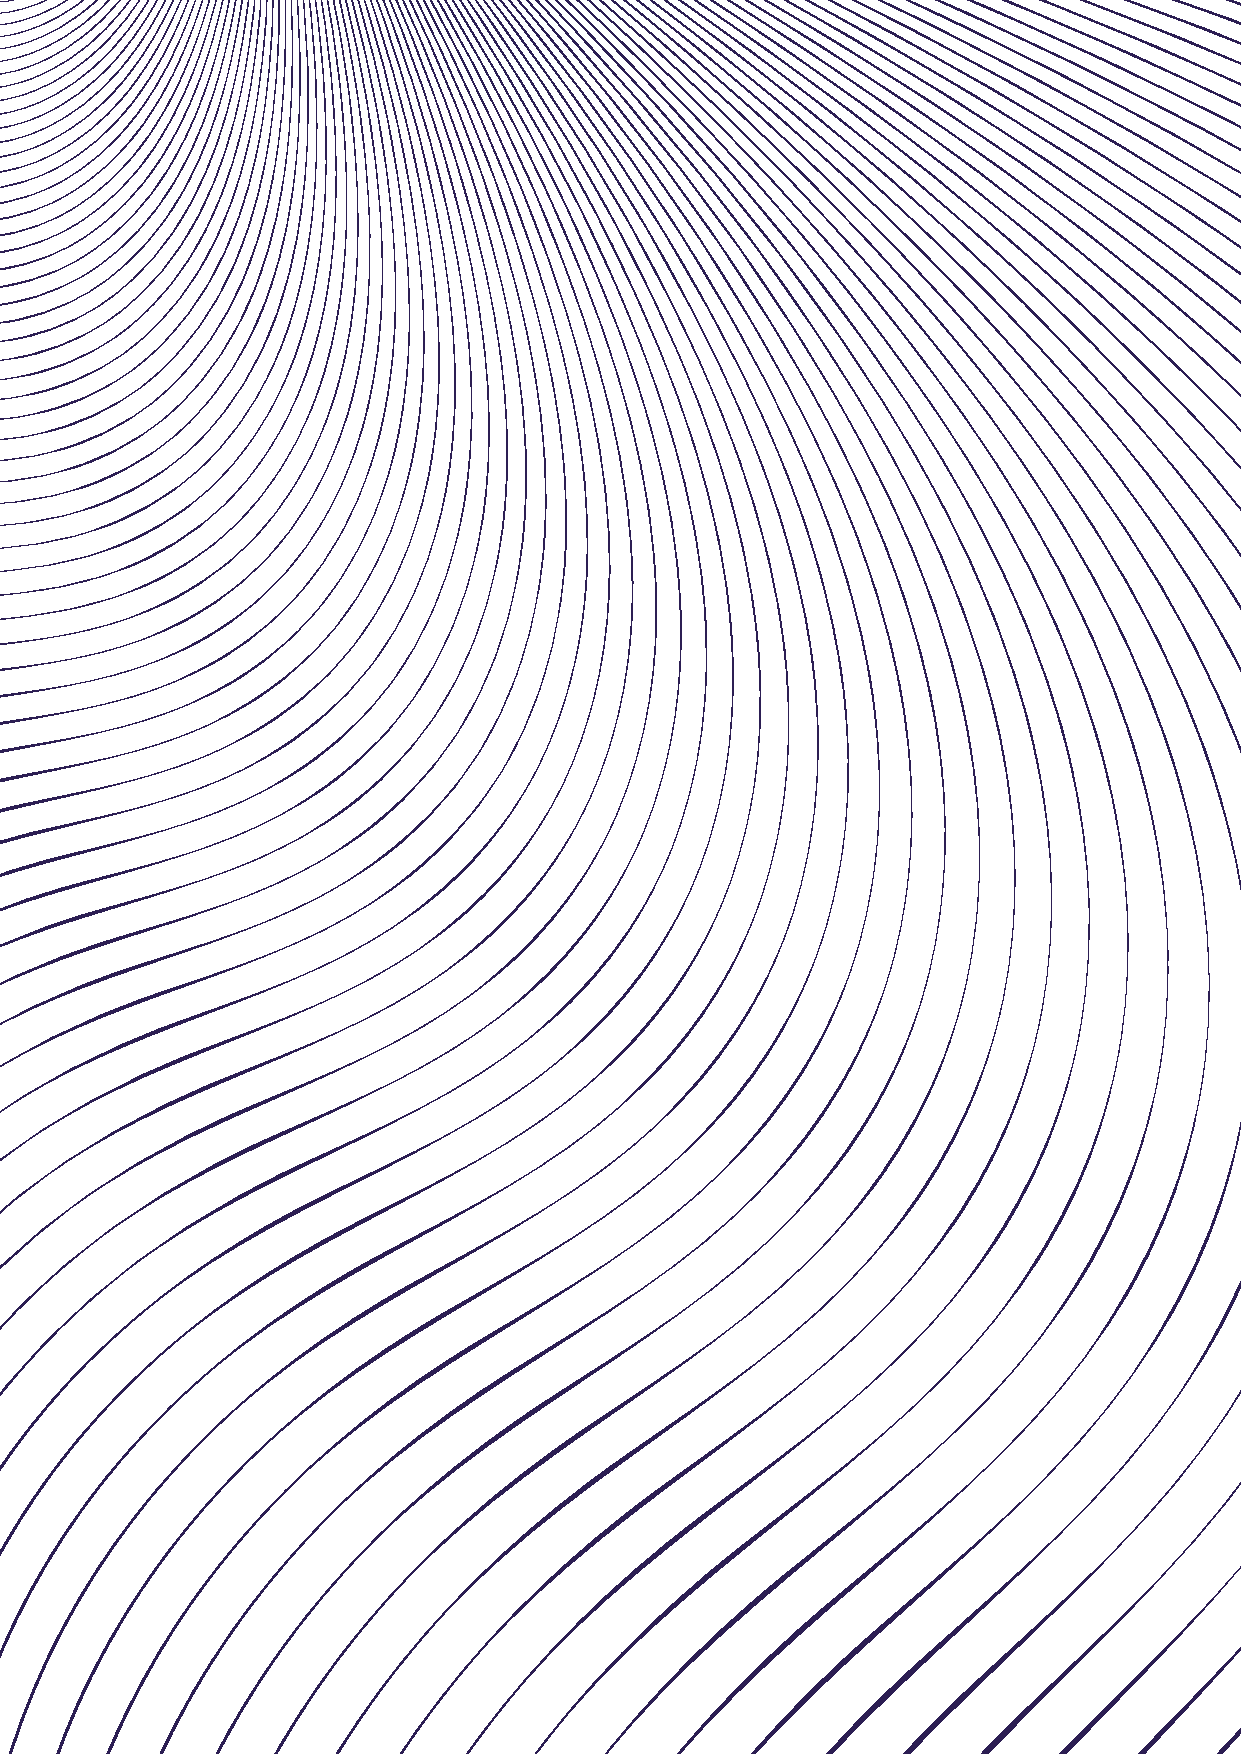
\includegraphics[width=\paperwidth,height=\paperheight]{aauGraphics/aau_waves}}}
  %\addtolength{\hoffset}{0.5\evensidemargin-0.5\oddsidemargin} %set equal margins on the frontpage - remove this line if you want default margins
  \noindent%
  % {\color{white}\fboxsep0pt\colorbox{aaublue}{\begin{tabular}{@{}p{\textwidth}@{}}
    \begin{center}
    \Huge{\textbf{
          Deep Learning Powered HAR Models
          }}
    \end{center}
    \begin{center}
      \Large{
      Forecasting the Realized Volatility of Bitcoin
      }
    \end{center}
    \vspace{0.2cm}
   \begin{center}
    {\Large
      Sebastian Tved Linde
    }\\
    \vspace{0.2cm}
    {\large
    Study No.: 20156272
    }\\
    \vspace{0.2cm}
    {\large
      Aalborg University Business School - M.Sc Finance
    }\\
   \vspace{0.2cm}
   {\large
   Supervisor: Frederik Steen Lundtofte, Full Professor of Finance 
   }

   \end{center}

   \vspace{0.2cm}
%% Comment this section in if you are doing Bachelor or Master Project   
   \begin{center}
    {\Large
     M.Sc Finance - Master's Thesis
    }\\
   \vspace{0.2cm}
   {\Large
   11-02-2022
   }
   \end{center}
  \vfill
  \begin{center}
    
\includegraphics[width=0.2\paperwidth]{aauGraphics/aau_logo_circle_en}% comment this line in for English version
  \end{center}
\end{titlepage}
\clearpage


\thispagestyle{empty}
\small
\strut\vfill
\noindent Copyright \copyright{} Aalborg University 2015\par
\vspace{0.2cm}
\noindent This project was created using Google Colab.\\
The notebook can be found at \href{https://colab.research.google.com/drive/1sJzRECcHC5H5JRsX7B5iEZdrGE-onn3X#scrollTo=RUfZZPrGUZoH}{Google Colab}.\\
\url{https://colab.research.google.com/drive/1sJzRECcHC5H5JRsX7B5iEZdrGE-onn3X?usp=sharing} \\
The computations done in Colab was done on a GPU, with a Colab Pro License.
\clearpage


\tableofcontents
